\documentclass[a4paper,12pt]{article}

%% Работа с русским языком
\usepackage{cmap}					% поиск в PDF
\usepackage{mathtext} 				% русские буквы в формулах
\usepackage[T2A]{fontenc}			% кодировка
\usepackage[utf8]{inputenc}			% кодировка исходного текста
\usepackage[english,russian]{babel}	% локализация и переносы

%% Отступы между абзацами и в начале абзаца 
\setlength{\parindent}{0pt}
\setlength{\parskip}{\medskipamount}

%% Изменяем размер полей
\usepackage[top=0.5in, bottom=0.75in, left=0.625in, right=0.625in]{geometry}

%% Графика
\usepackage[pdftex]{graphicx}
\graphicspath{{images/}}

%% Различные пакеты для работы с математикой
\usepackage{mathtools}				% Тот же amsmath, только с некоторыми поправками

\usepackage{amssymb}				% Математические символы
\usepackage{amsthm}					% Пакет для написания теорем
\usepackage{amstext}
\usepackage{array}
\usepackage{amsfonts}
\usepackage{icomma}					% "Умная" запятая: $0,2$ --- число, $0, 2$ --- перечисление
\usepackage{bbm}				    % Для красивого (!) \mathbb с  буквами и цифрами
\usepackage{enumitem}               % Для выравнивания itemise (\begin{itemize}[align=left])

% Номера формул
\mathtoolsset{showonlyrefs=true} % Показывать номера только у тех формул, на которые есть \eqref{} в тексте.

% Ссылки
\usepackage[colorlinks=true, urlcolor=blue]{hyperref}

% Шрифты
\usepackage{euscript}	 % Шрифт Евклид
\usepackage{mathrsfs}	 % Красивый матшрифт

% Свои команды\textbf{}
\DeclareMathOperator{\sgn}{\mathop{sgn}}

% Перенос знаков в формулах (по Львовскому)
\newcommand*{\hm}[1]{#1\nobreak\discretionary{}
{\hbox{$\mathsurround=0pt #1$}}{}}

% Графики
\usepackage{tikz}
\usepackage{pgfplots}
%\pgfplotsset{compat=1.12}

% Изменим формат \section и \subsection:
\usepackage{titlesec}
\titleformat{\section}
{\vspace{1cm}\centering\LARGE\bfseries}	% Стиль заголовка
{}										% префикс
{0pt}									% Расстояние между префиксом и заголовком
{} 										% Как отображается префикс
\titleformat{\subsection}				% Аналогично для \subsection
{\Large\bfseries}
{}
{0pt}
{}

% Информация об авторах
\author{Группа лектория ФКН ПМИ 2015-2016 \\
	Анастасия Иовлева \\
	Ксюша Закирова \\
	Руслан Хайдуров}
\title{Лекции по предмету \\
	\textbf{Линейная алгебра и геометрия}}
\date{2016 год}

\newtheorem*{Def}{Определение}
\newtheorem*{Lemma}{Лемма}
\newtheorem*{Suggestion}{Предложение}
\newtheorem*{Examples}{Пример}
\newtheorem*{Comment}{Замечание}
\newtheorem*{Consequence}{Следствие}
\newtheorem*{Theorem}{Теорема}
\newtheorem*{Statement}{Утверждение}
\newtheorem*{Task}{Упражнение}
\newtheorem*{Designation}{Обозначение}
\newtheorem*{Generalization}{Обобщение}
\newtheorem*{Thedream}{Предел мечтаний}
\newtheorem*{Properties}{Свойства}

\renewcommand{\mathbb}{\mathbbm}
\renewcommand{\Re}{\mathrm{Re\:}}
\renewcommand{\Im}{\mathrm{Im\:}}
\newcommand{\Arg}{\mathrm{Arg\:}}
\renewcommand{\arg}{\mathrm{arg\:}}
\newcommand{\Mat}{\mathrm{Mat}}
\newcommand{\id}{\mathrm{id}}
\newcommand{\isom}{\xrightarrow{\sim}} 
\newcommand{\leftisom}{\xleftarrow{\sim}}
\newcommand{\Hom}{\mathrm{Hom}}
\newcommand{\Ker}{\mathrm{Ker}\:}
\newcommand{\rk}{\mathrm{rk}\:}
\newcommand{\diag}{\mathrm{diag}}
\newcommand{\ort}{\mathrm{ort}}
\newcommand{\pr}{\mathrm{pr}}
\newcommand{\vol}{\mathrm{vol\:}}

\renewcommand{\epsilon}{\varepsilon}
\renewcommand{\phi}{\varphi}
\newcommand{\e}{\mathbb{e}}
\renewcommand{\l}{\lambda}
\renewcommand{\C}{\mathbb{C}}
\newcommand{\R}{\mathbb{R}}
\newcommand{\E}{\mathbb{E}}

\newcommand{\vvector}[1]{\begin{pmatrix}{#1}_1 \\\vdots\\{#1}_n\end{pmatrix}}
\renewcommand{\vector}[1]{({#1}_1, \ldots, {#1}_n)}

\begin{document}

\section*{Лекция 19 от 22.03.2016}

\subsection{Хорошая хеш-функция}

Пусть $H$ --- семейство хеш-функций $h: U \to \{0, 1, \ldots, m-1\}$. Назовём $H$ \emph{универсальной}, если выплолняется
\[\forall x\in U, y\in U \left|\left\{ h(x) = h(y)\mid h\in H \right\}\right| = \frac{|H|}{m}\]

При случайном выборе $h\in H$ $\mathrm{Pr}[h(x) = h(y)] = \frac{1}{m}$

Будем считать, что пользуемся такой $h$.

Пусть $m = n^2$, где $n$ --- число хранимых ключей. Выберем $h\in H$; сколько будет коллизий (таких пар $(x, y)$, что $h(x) = h(y)$)? Утверждается, что немного.

Давайте оценим матожидание коллизии:

\[
    E(\text{число коллизий}) = Pr(\text{коллизия})*{n \choose 2} = \frac{1}{m}\cdot\frac{n(n-1)}{2} = \frac{n-1}{2n}<\frac{1}{2}
\]

\[
    Pr(\text{\# коллизий} \geqslant 1) \leqslant \frac{ E(\text{\# коллизий})}{1} = \frac{1}{2}
\]

\[
    Pr(\text{коллизий нет}) \geqslant \frac{1}{2}
\]

Заметим, что тогда (мы опираемся на то, что данные сохраняются единожды) получается, что потратив в среднем две попытки мы можем найти такую $h$, что хеширование произойдёт без коллизий и поиск будет за константное время (это, кстати, называется \emph{идеальным хешированием}).

Или давайте так:

Создадим таблицу из $m = n$ ячеек; но таблица будет не простой, а состоящей из хеш-таблиц; при этом внутри каждой такой таблицы коллизий не будет (мы об этом позаботимся).

Пусть $n_j$ --- число элементов таких, что $h(x) = j$. $\sum\limits_j n_j = n$, как несложно заметить. Введём также $m_j$ --- число ячеек в $j$-ой таблице второго уровня. Если мы хотим обеспечить отсутствие коллизий (и не потратить на это кучу времени), то $m_j$ должно быть равно $n_j^2$. Вопрос --- а чем такой способ лучше предыдущего? А давайте посмотрим на память: внешняя таблица имеет линейное количество ячеек, где каждая имеет константную память (там хранятся лишь ссылки на таблицы второго уровня). А память на таблицы второго уровня --- $\sum\limits_{j=0}^{m-1} \Theta(n_j^2)$. Понятно, что если придумать худший случай, то все будут в одной ячейке. Давайте тогда считать матожидание:

\[
    E\left[ \sum\limits_{j=0}^{m-1} \Theta(n_j^2) \right]
\]

Но сначала вот что:

\[
    n_j^2 = n_j +n_j^2 - n_j = n_j+n_j(n_j-1) = n_j + 2{n_j \choose 2}
\]

\begin{multline*}
    E\left[ \sum\limits_{j=0}^{m-1} n_j^2 \right] = 
    E\left[ \sum\limits_{j=0}^{m-1} n_j + 2{n_j \choose 2} \right] = 
    E\left[ \sum\limits_{j=0}^{m-1} n_j \right] + 2E\left[{n_j \choose 2} \right] = \\ =
    n + 2E\left[ \text{\# коллизий для $h$} \right] \leqslant
    n + 2\cdot\frac{1}{m}\cdot\frac{n(n-1)}{2} =
    n + n - 1 =
    2n - 1
\end{multline*}

Ой! Линейная память! Вот и искомое преимущество.

Но пока всё довольно абстрактно. Где брать такие универсальные хеш-функции? Давайте приведём пример:

Рассмотрим $H_{p\, m}$, где $p$ --- простое число, большее всех ключей.
Пусть она состоит из функций $h(k) = \left( \left( ak+b \right)\mod{p} \right)\mod{m};\ a\in[1;p],\ b\in[0; p]$

\subsection{Красно-чёрное дерево}

Что такое бинарное дерево поиска мы знаем; рассмотрим теперь \emph{сбалансированное} бинарное дерево. Его ключевое свойство: высота такого дерева --- $O(\log n)$. Разумеется, речь идёт о семействе деревьев; сказать, выполняется ли это для конкретного дерева нельзя.

Рассмотрим один класс таких деревьев --- \emph{красно-чёрные} деревья. Ключевые характеристики:

\begin{enumerate}
    \item Любой узел --- красный или чёрный.
    \item Корень и листья --- чёрные.
    \item Родителем красного узла может быть только чёрный.
    \item На всех простых путях из узла $x$ до листьев-наследников одинаковое количество чёрных узлов.
\end{enumerate}

Вот как может выглядеть такое дерево:

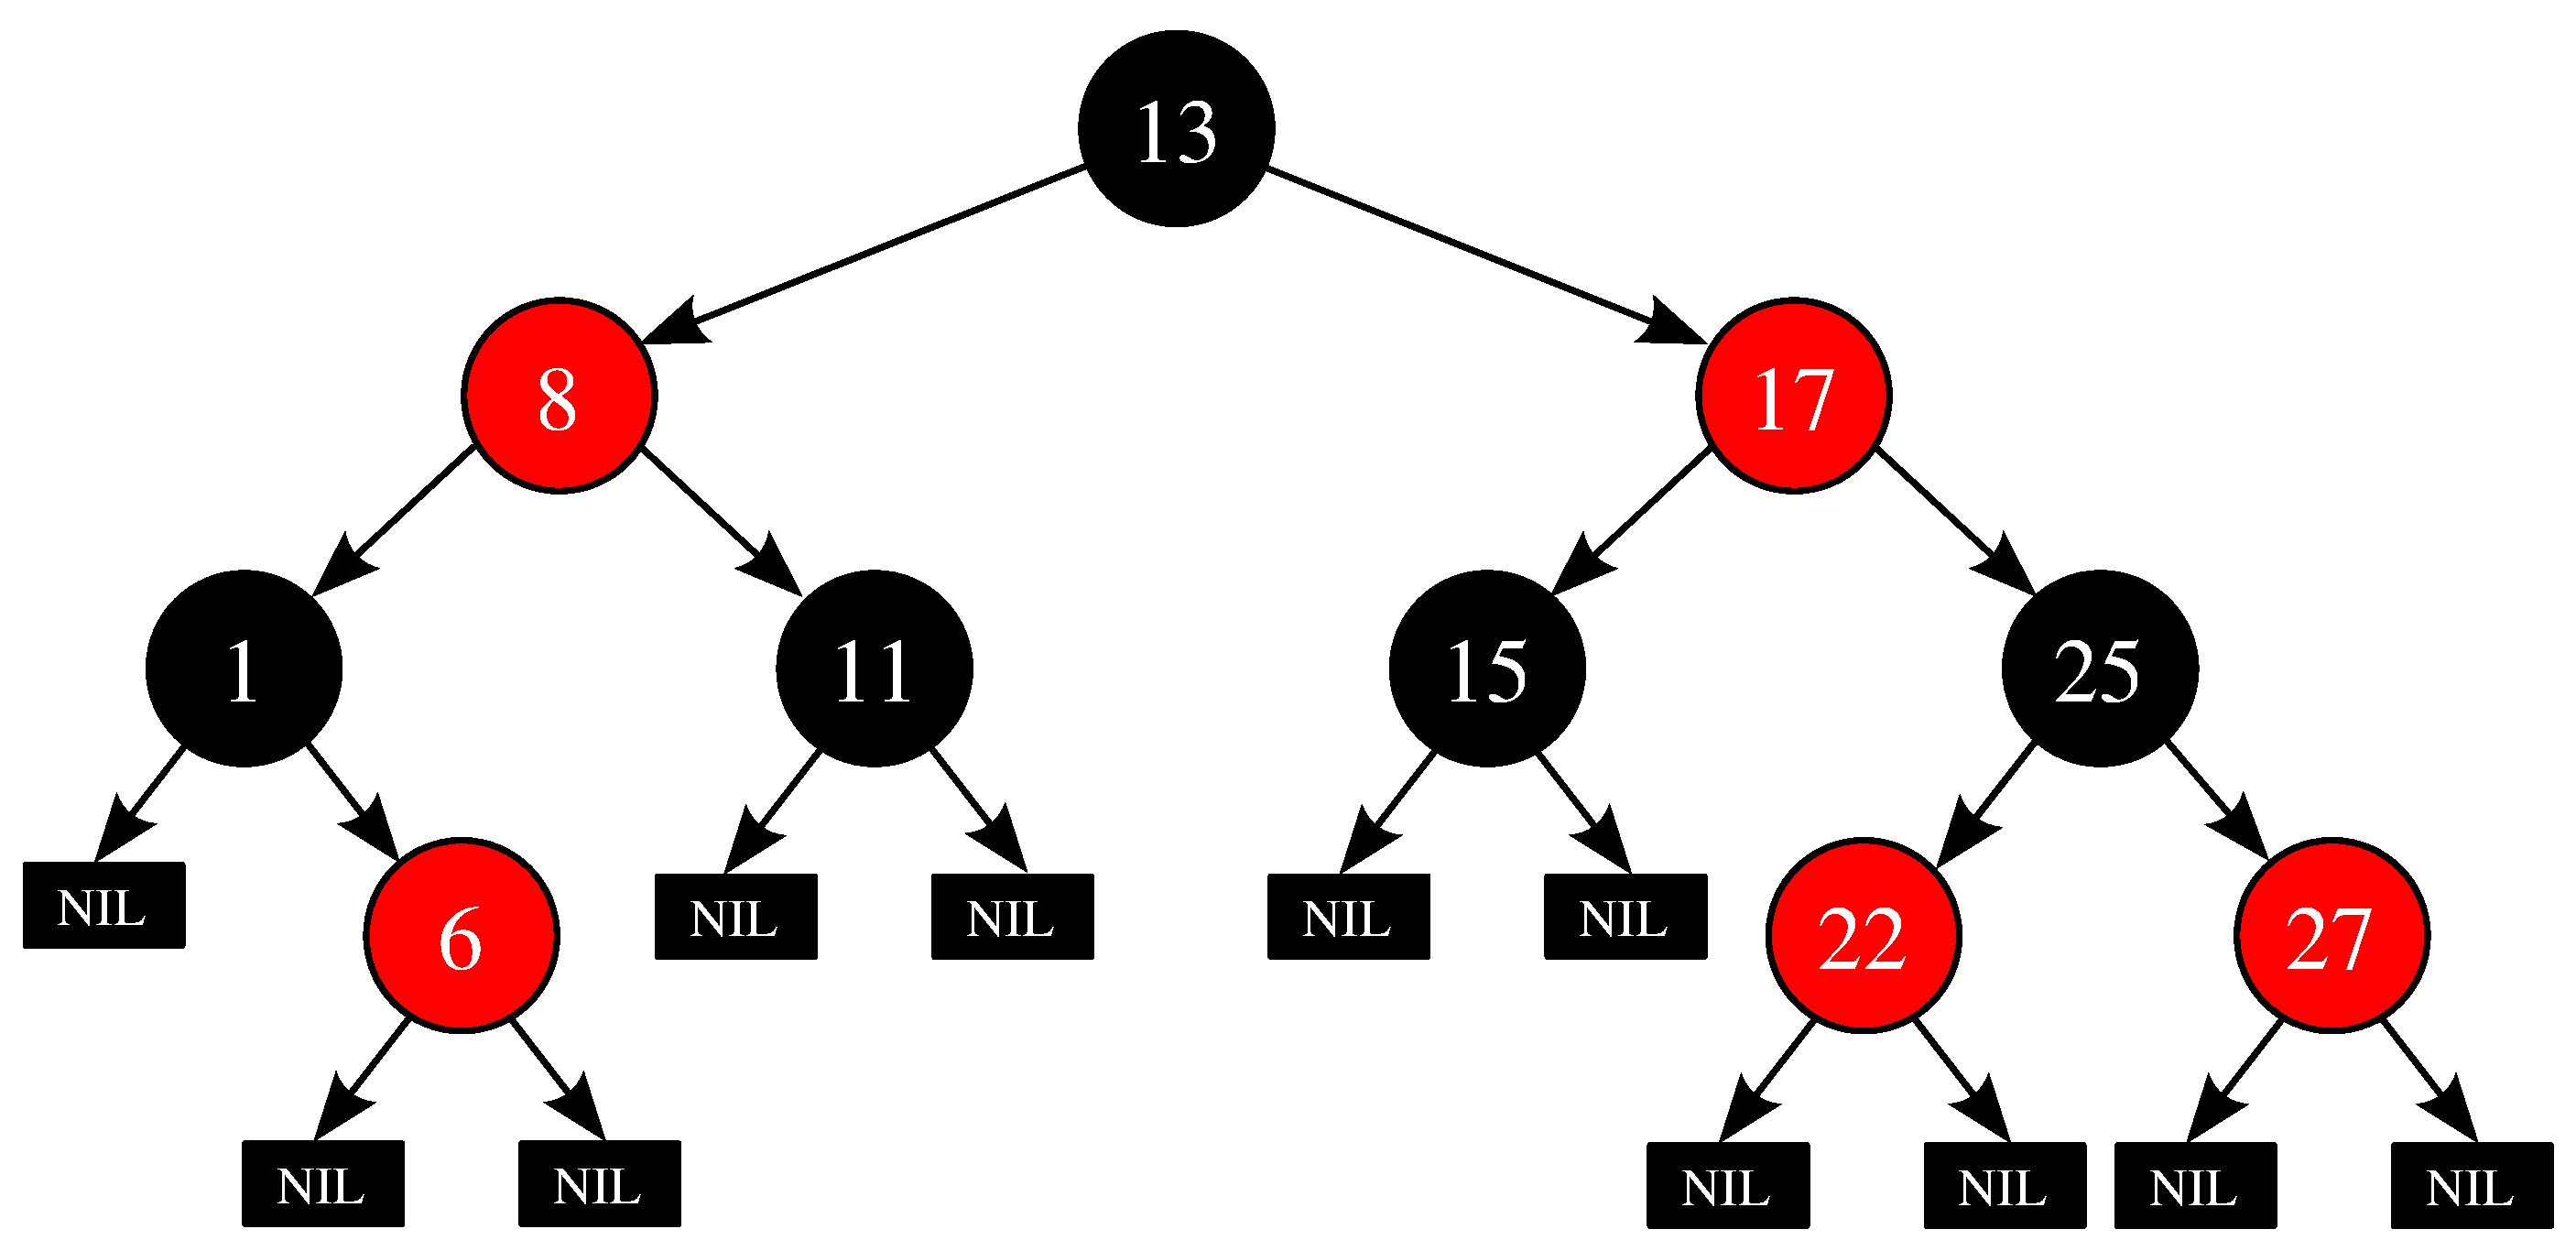
\includegraphics[width=15cm]{images/19_rb_tree.pdf}

Высота RB-дерева с $n$ ключами не больше $2\log_2(n+1)$. Докажем это не вполне формально:

``Подтянем'' красные узлы к чёрным родителям. Легко заметить, что высота дерева уменьшилась не больше, чем вдвое: $n \leqslant 2h'$. Число листьев, получившихся в итоге --- $n+1 \geqslant 2^{h'}$; $\log_2(n+1)\geqslant h'\geqslant\frac{h}{2}$. Значит, высота дерева --- $O(\log n)$ и поиск в дереве займёт логарифмическое время.

\begin{lstlisting}
rb_insert(t, x):
    tree_insert(t, x)
    x.color = 'red'
    while x != t.root and x.p.color = 'red' do
        if x.p = x.p.p.right then
            y:= x.p.p.left
            if y.color = 'red' then
                x.p.color:= 'black'
                y.color:= 'black'
                x.p.p.color = 'red'
            else
                AAAAAAAAAAAA
\end{lstlisting}
\end{document}
